\documentclass[12pt, a4paper]{article}

\usepackage[utf8]{inputenc}
\usepackage[T1]{fontenc}
\usepackage[brazilian]{babel}
\usepackage{mathptmx}
\usepackage{amsmath, amssymb}
\usepackage{graphicx}
\usepackage{booktabs}
\usepackage{geometry}
\usepackage{float}
\usepackage{setspace}
\usepackage{caption}

\geometry{top=3cm, bottom=2cm, left=3cm, right=2cm}
\setstretch{1.5}
\captionsetup{font=small, labelfont=bf, labelsep=endash}

\begin{document}

\begin{center}
    \Large\textbf{Relatório Consolidado de Benchmarking -- Iniciação Científica} \\[0.2cm]
    \large\textit{Escalabilidade de Hardware vs. Estruturação Física de Dados (DataOps) no Apache Druid} \\[0.5cm]
    \normalsize\textbf{Projeto DataOps / UNIFEI} \\
    \small{\today}
\end{center}

\vspace{0.5cm}
\noindent\rule{\textwidth}{1pt}

\section*{1. Resumo Executivo da Metodologia}
Este documento unifica as seis etapas da pesquisa experimental. O objetivo foi quantificar o impacto da paralelização de hardware (2, 4 e 6 núcleos) em contraponto à aplicação de técnicas de \textit{DataOps} (neste caso, a compactação de dados). A base total compreende mais de 3,1 milhões de registros de focos de calor, inicialmente distribuídos em 6.518 arquivos minúsculos (\textit{Tiny Segments}) e, posteriormente, compactados com granularidade anual (\textit{CompactYear}).

\section*{2. Fase 1: O Gargalo da Fragmentação (Cenários 1 a 3)}
No \textbf{Cenário 1} (2 Núcleos, Fragmentado), o sistema operou sob estrangulamento severo de I/O. As latências de varredura plena superaram a marca crítica dos \textbf{4666.32 ms}. Registrou-se o início do Paradoxo do Cache, onde a consulta territorial obteve otimização negativa (\textbf{-0.76\%}).

Com o \textbf{Cenário 2} (4 Núcleos) e \textbf{Cenário 3} (6 Núcleos), o incremento bruto de processador atenuou a latência. A Alta Cardinalidade caiu para \textbf{1756.32 ms} no ápice do hospedeiro. Contudo, a ineficiência do cache colunar persistiu (\textbf{-12.47\%} em C3), provando que injetar processador não resolve o gargalo de roteamento lógico em memória RAM causado pela fragmentação.

\begin{figure}[H]
\centering
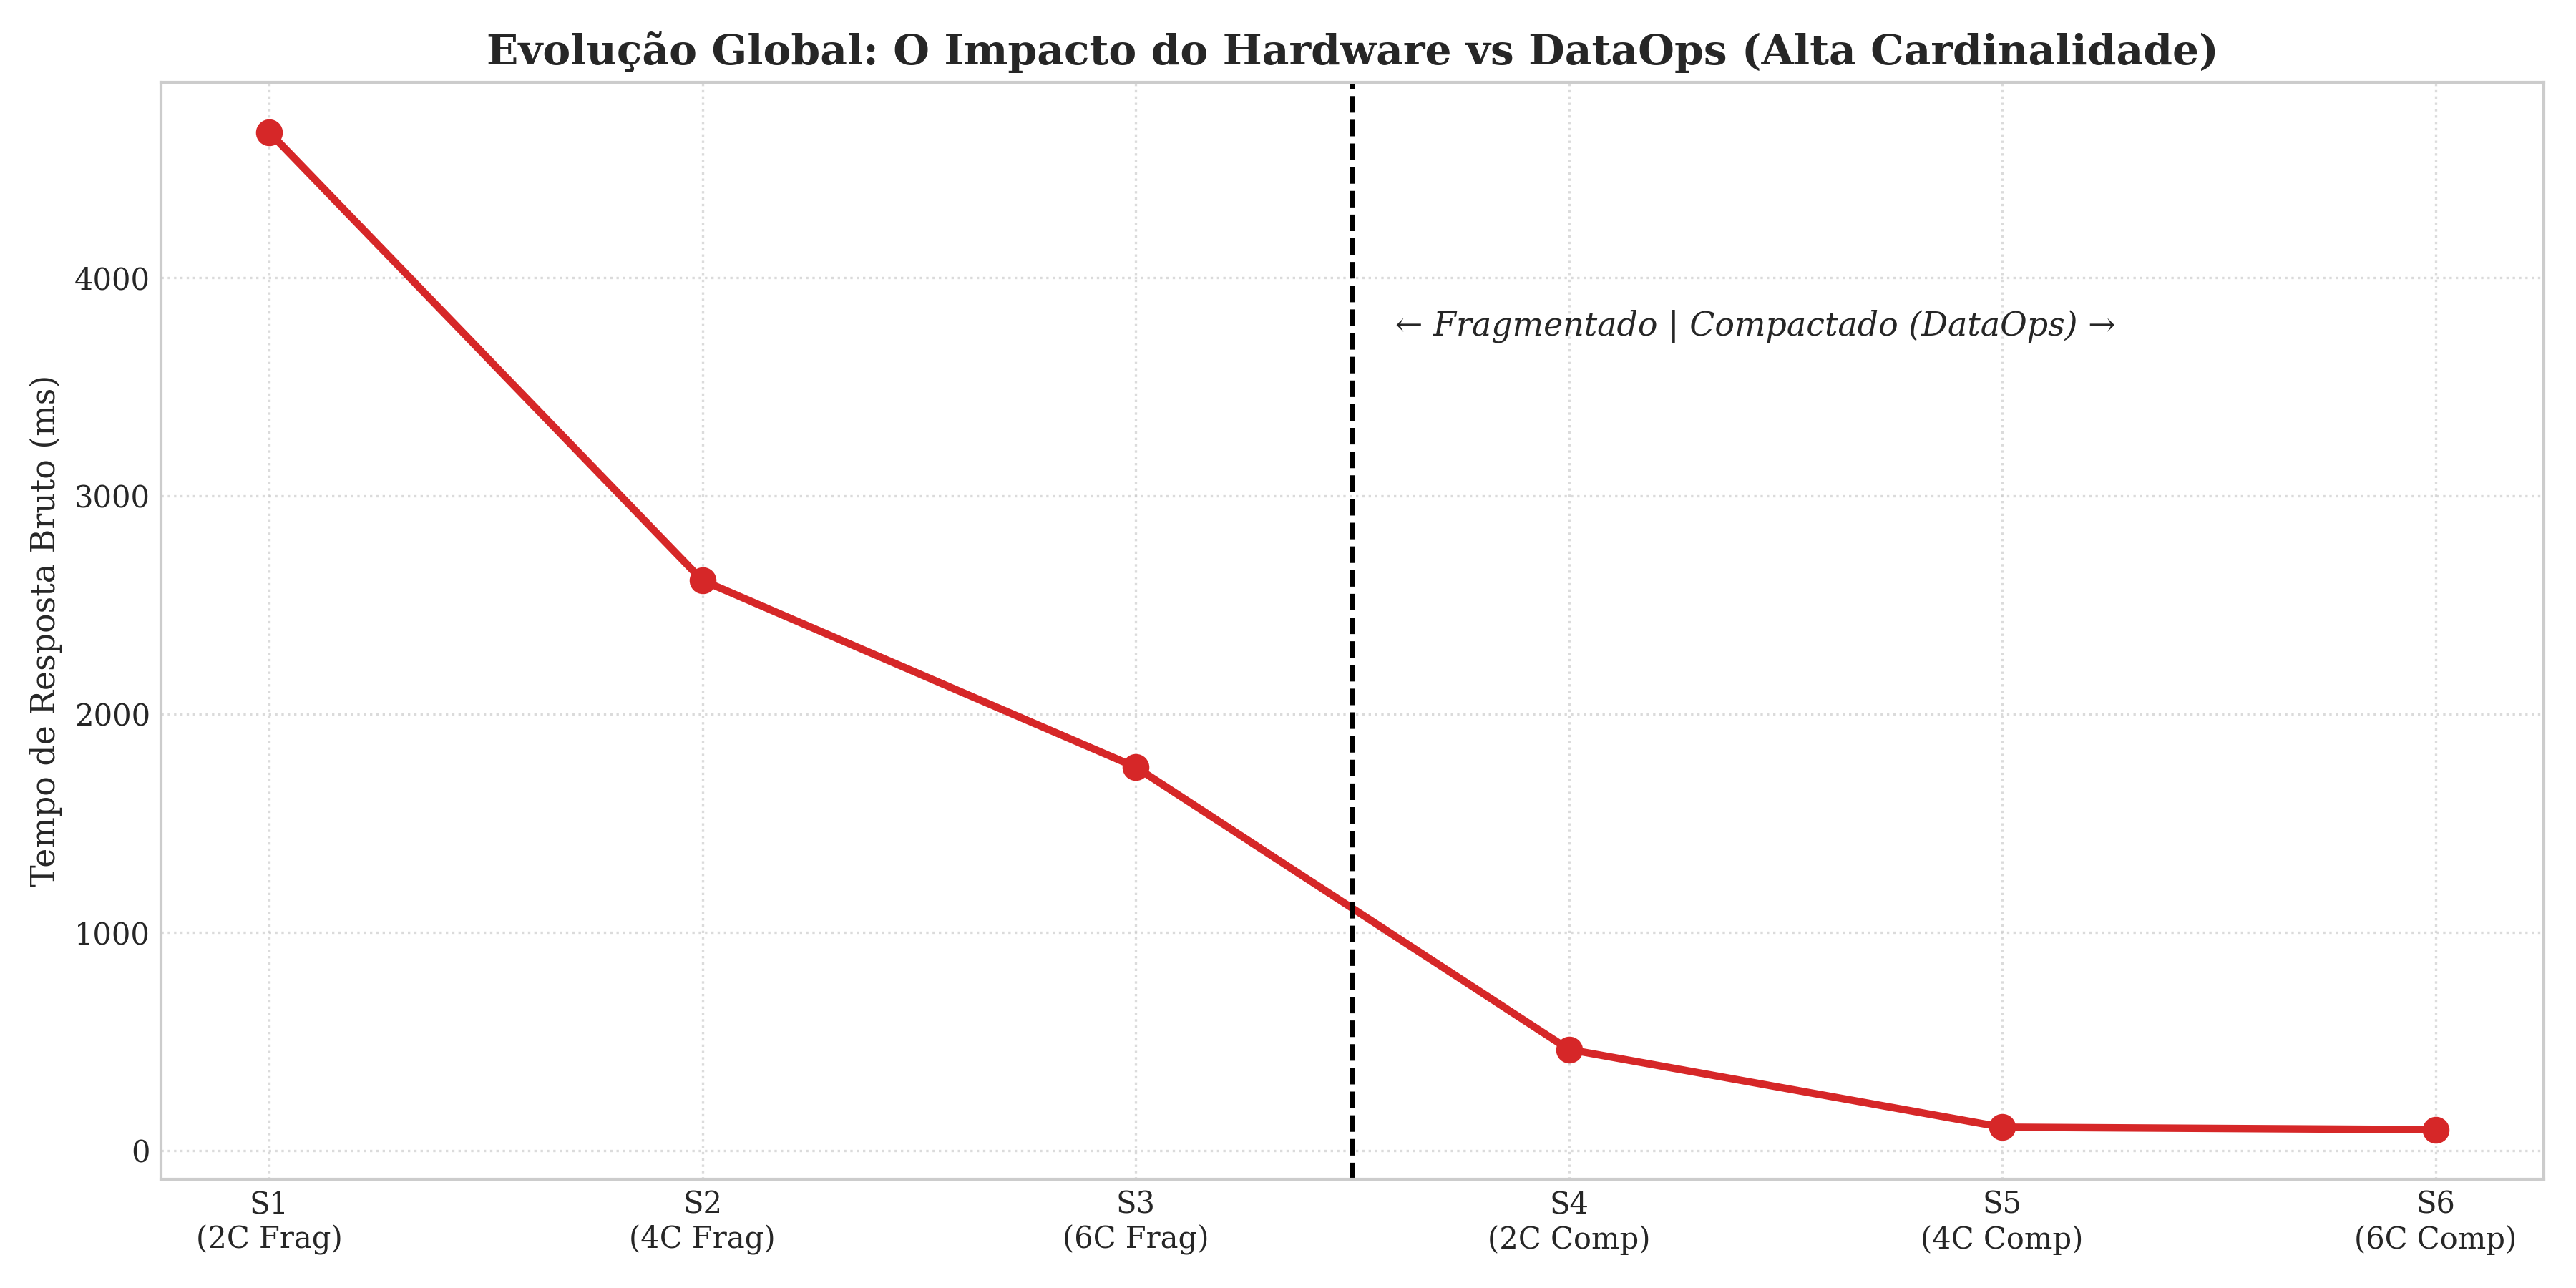
\includegraphics[width=0.95\textwidth]{fig_evolucao_global.png}
\caption{A evolução contundente do tempo de resposta provando a superioridade do DataOps sobre o provisonamento de hardware bruto.}
\end{figure}

\section*{3. Fase 2: O Triunfo do DataOps (Cenários 4 a 6)}
A virada arquitetural ocorreu no \textbf{Cenário 4}, onde o hardware foi rebaixado para 2 núcleos, mas a base foi consolidada via \textit{Compaction}. A latência de Alta Cardinalidade despencou de forma colossal para \textbf{461.91 ms}. O cache RAM ressuscitou, atingindo picos de eficiência de \textbf{87.76\%}.

Ao aplicar paralelismo sobre a base otimizada no \textbf{Cenário 5} (4 núcleos) e \textbf{Cenário 6} (6 núcleos), o sistema atingiu seu limite fisiológico. No Cenário 6, a Alta Cardinalidade quebrou a barreira dos 100ms, registrando \textbf{94.45 ms}. 

O fenômeno mais intrigante, o \textit{``Too Fast to Cache''}, atingiu seu extremo no Cenário 6. Consultas complexas demoraram apenas \textbf{18.91 ms} no processamento bruto, tornando-se mais rápidas que a própria memória RAM (\textbf{27.90 ms}), o que gerou um ganho matemático negativo de \textbf{-47.54\%}.

\section*{4. Conclusão da Pesquisa}
A bateria de testes comprova matematicamente a hipótese central: em bancos de dados analíticos colunares orientados a \textit{Big Data} (OLAP), a engenharia física dos dados supera amplamente o provisionamento irrestrito de CPU. A compactação reduziu o tempo de resposta em mais de 40 vezes, enquanto a adição de núcleos entregou ganhos secundários de refino.

\end{document}
